\begin{figure*}[h]
  \centering
  % 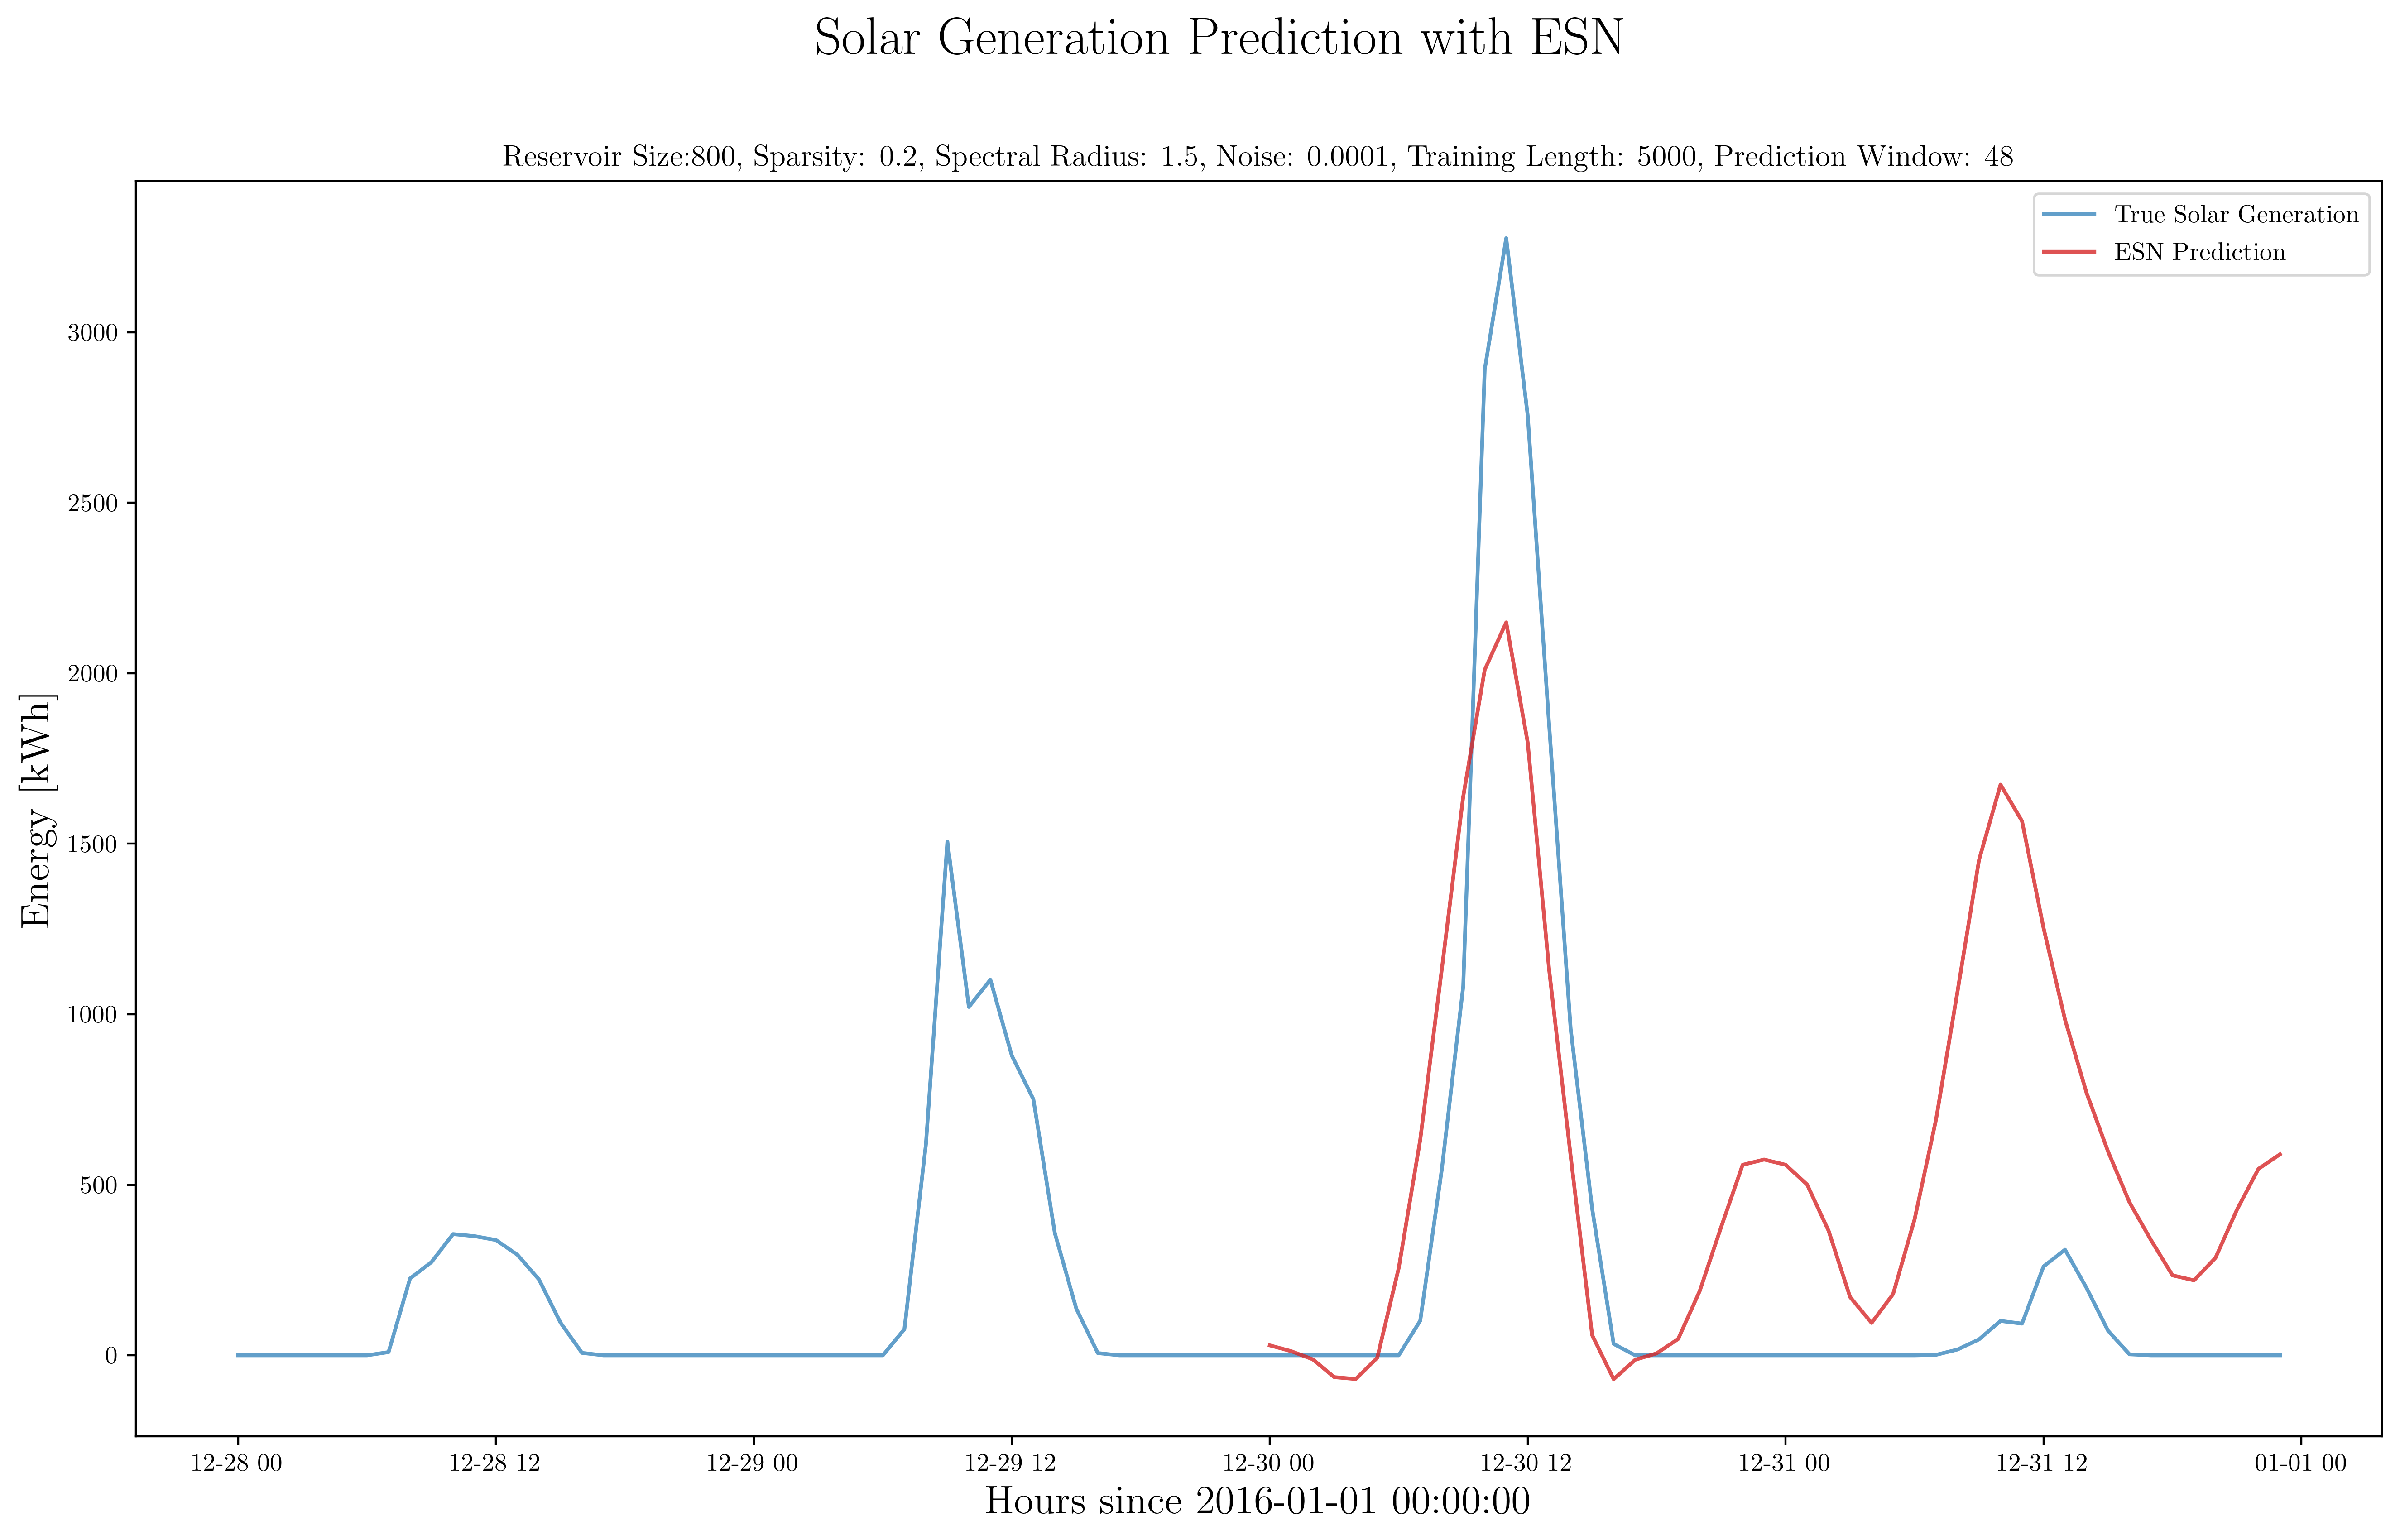
\includegraphics[width=0.8\textwidth]{48_solar_humidity_prediction.png}
  %% Creator: Matplotlib, PGF backend
%%
%% To include the figure in your LaTeX document, write
%%   \input{<filename>.pgf}
%%
%% Make sure the required packages are loaded in your preamble
%%   \usepackage{pgf}
%%
%% Figures using additional raster images can only be included by \input if
%% they are in the same directory as the main LaTeX file. For loading figures
%% from other directories you can use the `import` package
%%   \usepackage{import}
%% and then include the figures with
%%   \import{<path to file>}{<filename>.pgf}
%%
%% Matplotlib used the following preamble
%%
\begingroup%
\makeatletter%
\begin{pgfpicture}%
\pgfpathrectangle{\pgfpointorigin}{\pgfqpoint{5.531696in}{3.164528in}}%
\pgfusepath{use as bounding box, clip}%
\begin{pgfscope}%
\pgfsetbuttcap%
\pgfsetmiterjoin%
\definecolor{currentfill}{rgb}{1.000000,1.000000,1.000000}%
\pgfsetfillcolor{currentfill}%
\pgfsetlinewidth{0.000000pt}%
\definecolor{currentstroke}{rgb}{1.000000,1.000000,1.000000}%
\pgfsetstrokecolor{currentstroke}%
\pgfsetdash{}{0pt}%
\pgfpathmoveto{\pgfqpoint{0.000000in}{0.000000in}}%
\pgfpathlineto{\pgfqpoint{5.531696in}{0.000000in}}%
\pgfpathlineto{\pgfqpoint{5.531696in}{3.164528in}}%
\pgfpathlineto{\pgfqpoint{0.000000in}{3.164528in}}%
\pgfpathclose%
\pgfusepath{fill}%
\end{pgfscope}%
\begin{pgfscope}%
\pgfsetbuttcap%
\pgfsetmiterjoin%
\definecolor{currentfill}{rgb}{1.000000,1.000000,1.000000}%
\pgfsetfillcolor{currentfill}%
\pgfsetlinewidth{0.000000pt}%
\definecolor{currentstroke}{rgb}{0.000000,0.000000,0.000000}%
\pgfsetstrokecolor{currentstroke}%
\pgfsetstrokeopacity{0.000000}%
\pgfsetdash{}{0pt}%
\pgfpathmoveto{\pgfqpoint{0.669445in}{0.499691in}}%
\pgfpathlineto{\pgfqpoint{5.431696in}{0.499691in}}%
\pgfpathlineto{\pgfqpoint{5.431696in}{2.865455in}}%
\pgfpathlineto{\pgfqpoint{0.669445in}{2.865455in}}%
\pgfpathclose%
\pgfusepath{fill}%
\end{pgfscope}%
\begin{pgfscope}%
\pgfpathrectangle{\pgfqpoint{0.669445in}{0.499691in}}{\pgfqpoint{4.762251in}{2.365763in}}%
\pgfusepath{clip}%
\pgfsetbuttcap%
\pgfsetroundjoin%
\definecolor{currentfill}{rgb}{0.501961,0.501961,0.501961}%
\pgfsetfillcolor{currentfill}%
\pgfsetfillopacity{0.600000}%
\pgfsetlinewidth{1.003750pt}%
\definecolor{currentstroke}{rgb}{0.501961,0.501961,0.501961}%
\pgfsetstrokecolor{currentstroke}%
\pgfsetstrokeopacity{0.600000}%
\pgfsetdash{}{0pt}%
\pgfpathmoveto{\pgfqpoint{3.164500in}{0.644727in}}%
\pgfpathlineto{\pgfqpoint{3.164500in}{0.652309in}}%
\pgfpathlineto{\pgfqpoint{3.210072in}{0.652309in}}%
\pgfpathlineto{\pgfqpoint{3.255644in}{0.652309in}}%
\pgfpathlineto{\pgfqpoint{3.301216in}{0.652309in}}%
\pgfpathlineto{\pgfqpoint{3.301216in}{0.647631in}}%
\pgfpathlineto{\pgfqpoint{3.301216in}{0.647631in}}%
\pgfpathlineto{\pgfqpoint{3.255644in}{0.607625in}}%
\pgfpathlineto{\pgfqpoint{3.210072in}{0.611187in}}%
\pgfpathlineto{\pgfqpoint{3.164500in}{0.644727in}}%
\pgfpathclose%
\pgfusepath{stroke,fill}%
\end{pgfscope}%
\begin{pgfscope}%
\pgfpathrectangle{\pgfqpoint{0.669445in}{0.499691in}}{\pgfqpoint{4.762251in}{2.365763in}}%
\pgfusepath{clip}%
\pgfsetbuttcap%
\pgfsetroundjoin%
\definecolor{currentfill}{rgb}{0.501961,0.501961,0.501961}%
\pgfsetfillcolor{currentfill}%
\pgfsetfillopacity{0.600000}%
\pgfsetlinewidth{1.003750pt}%
\definecolor{currentstroke}{rgb}{0.501961,0.501961,0.501961}%
\pgfsetstrokecolor{currentstroke}%
\pgfsetstrokeopacity{0.600000}%
\pgfsetdash{}{0pt}%
\pgfpathmoveto{\pgfqpoint{3.802505in}{0.607226in}}%
\pgfpathlineto{\pgfqpoint{3.802505in}{0.652309in}}%
\pgfpathlineto{\pgfqpoint{3.848077in}{0.652309in}}%
\pgfpathlineto{\pgfqpoint{3.848077in}{0.643862in}}%
\pgfpathlineto{\pgfqpoint{3.848077in}{0.643862in}}%
\pgfpathlineto{\pgfqpoint{3.802505in}{0.607226in}}%
\pgfpathclose%
\pgfusepath{stroke,fill}%
\end{pgfscope}%
\begin{pgfscope}%
\pgfsetbuttcap%
\pgfsetroundjoin%
\definecolor{currentfill}{rgb}{0.000000,0.000000,0.000000}%
\pgfsetfillcolor{currentfill}%
\pgfsetlinewidth{0.803000pt}%
\definecolor{currentstroke}{rgb}{0.000000,0.000000,0.000000}%
\pgfsetstrokecolor{currentstroke}%
\pgfsetdash{}{0pt}%
\pgfsys@defobject{currentmarker}{\pgfqpoint{0.000000in}{-0.048611in}}{\pgfqpoint{0.000000in}{0.000000in}}{%
\pgfpathmoveto{\pgfqpoint{0.000000in}{0.000000in}}%
\pgfpathlineto{\pgfqpoint{0.000000in}{-0.048611in}}%
\pgfusepath{stroke,fill}%
}%
\begin{pgfscope}%
\pgfsys@transformshift{1.432773in}{0.499691in}%
\pgfsys@useobject{currentmarker}{}%
\end{pgfscope}%
\end{pgfscope}%
\begin{pgfscope}%
\definecolor{textcolor}{rgb}{0.000000,0.000000,0.000000}%
\pgfsetstrokecolor{textcolor}%
\pgfsetfillcolor{textcolor}%
\pgftext[x=1.432773in,y=0.402469in,,top]{\color{textcolor}\rmfamily\fontsize{10.000000}{12.000000}\selectfont \(\displaystyle 26220\)}%
\end{pgfscope}%
\begin{pgfscope}%
\pgfsetbuttcap%
\pgfsetroundjoin%
\definecolor{currentfill}{rgb}{0.000000,0.000000,0.000000}%
\pgfsetfillcolor{currentfill}%
\pgfsetlinewidth{0.803000pt}%
\definecolor{currentstroke}{rgb}{0.000000,0.000000,0.000000}%
\pgfsetstrokecolor{currentstroke}%
\pgfsetdash{}{0pt}%
\pgfsys@defobject{currentmarker}{\pgfqpoint{0.000000in}{-0.048611in}}{\pgfqpoint{0.000000in}{0.000000in}}{%
\pgfpathmoveto{\pgfqpoint{0.000000in}{0.000000in}}%
\pgfpathlineto{\pgfqpoint{0.000000in}{-0.048611in}}%
\pgfusepath{stroke,fill}%
}%
\begin{pgfscope}%
\pgfsys@transformshift{2.344208in}{0.499691in}%
\pgfsys@useobject{currentmarker}{}%
\end{pgfscope}%
\end{pgfscope}%
\begin{pgfscope}%
\definecolor{textcolor}{rgb}{0.000000,0.000000,0.000000}%
\pgfsetstrokecolor{textcolor}%
\pgfsetfillcolor{textcolor}%
\pgftext[x=2.344208in,y=0.402469in,,top]{\color{textcolor}\rmfamily\fontsize{10.000000}{12.000000}\selectfont \(\displaystyle 26240\)}%
\end{pgfscope}%
\begin{pgfscope}%
\pgfsetbuttcap%
\pgfsetroundjoin%
\definecolor{currentfill}{rgb}{0.000000,0.000000,0.000000}%
\pgfsetfillcolor{currentfill}%
\pgfsetlinewidth{0.803000pt}%
\definecolor{currentstroke}{rgb}{0.000000,0.000000,0.000000}%
\pgfsetstrokecolor{currentstroke}%
\pgfsetdash{}{0pt}%
\pgfsys@defobject{currentmarker}{\pgfqpoint{0.000000in}{-0.048611in}}{\pgfqpoint{0.000000in}{0.000000in}}{%
\pgfpathmoveto{\pgfqpoint{0.000000in}{0.000000in}}%
\pgfpathlineto{\pgfqpoint{0.000000in}{-0.048611in}}%
\pgfusepath{stroke,fill}%
}%
\begin{pgfscope}%
\pgfsys@transformshift{3.255644in}{0.499691in}%
\pgfsys@useobject{currentmarker}{}%
\end{pgfscope}%
\end{pgfscope}%
\begin{pgfscope}%
\definecolor{textcolor}{rgb}{0.000000,0.000000,0.000000}%
\pgfsetstrokecolor{textcolor}%
\pgfsetfillcolor{textcolor}%
\pgftext[x=3.255644in,y=0.402469in,,top]{\color{textcolor}\rmfamily\fontsize{10.000000}{12.000000}\selectfont \(\displaystyle 26260\)}%
\end{pgfscope}%
\begin{pgfscope}%
\pgfsetbuttcap%
\pgfsetroundjoin%
\definecolor{currentfill}{rgb}{0.000000,0.000000,0.000000}%
\pgfsetfillcolor{currentfill}%
\pgfsetlinewidth{0.803000pt}%
\definecolor{currentstroke}{rgb}{0.000000,0.000000,0.000000}%
\pgfsetstrokecolor{currentstroke}%
\pgfsetdash{}{0pt}%
\pgfsys@defobject{currentmarker}{\pgfqpoint{0.000000in}{-0.048611in}}{\pgfqpoint{0.000000in}{0.000000in}}{%
\pgfpathmoveto{\pgfqpoint{0.000000in}{0.000000in}}%
\pgfpathlineto{\pgfqpoint{0.000000in}{-0.048611in}}%
\pgfusepath{stroke,fill}%
}%
\begin{pgfscope}%
\pgfsys@transformshift{4.167079in}{0.499691in}%
\pgfsys@useobject{currentmarker}{}%
\end{pgfscope}%
\end{pgfscope}%
\begin{pgfscope}%
\definecolor{textcolor}{rgb}{0.000000,0.000000,0.000000}%
\pgfsetstrokecolor{textcolor}%
\pgfsetfillcolor{textcolor}%
\pgftext[x=4.167079in,y=0.402469in,,top]{\color{textcolor}\rmfamily\fontsize{10.000000}{12.000000}\selectfont \(\displaystyle 26280\)}%
\end{pgfscope}%
\begin{pgfscope}%
\pgfsetbuttcap%
\pgfsetroundjoin%
\definecolor{currentfill}{rgb}{0.000000,0.000000,0.000000}%
\pgfsetfillcolor{currentfill}%
\pgfsetlinewidth{0.803000pt}%
\definecolor{currentstroke}{rgb}{0.000000,0.000000,0.000000}%
\pgfsetstrokecolor{currentstroke}%
\pgfsetdash{}{0pt}%
\pgfsys@defobject{currentmarker}{\pgfqpoint{0.000000in}{-0.048611in}}{\pgfqpoint{0.000000in}{0.000000in}}{%
\pgfpathmoveto{\pgfqpoint{0.000000in}{0.000000in}}%
\pgfpathlineto{\pgfqpoint{0.000000in}{-0.048611in}}%
\pgfusepath{stroke,fill}%
}%
\begin{pgfscope}%
\pgfsys@transformshift{5.078515in}{0.499691in}%
\pgfsys@useobject{currentmarker}{}%
\end{pgfscope}%
\end{pgfscope}%
\begin{pgfscope}%
\definecolor{textcolor}{rgb}{0.000000,0.000000,0.000000}%
\pgfsetstrokecolor{textcolor}%
\pgfsetfillcolor{textcolor}%
\pgftext[x=5.078515in,y=0.402469in,,top]{\color{textcolor}\rmfamily\fontsize{10.000000}{12.000000}\selectfont \(\displaystyle 26300\)}%
\end{pgfscope}%
\begin{pgfscope}%
\definecolor{textcolor}{rgb}{0.000000,0.000000,0.000000}%
\pgfsetstrokecolor{textcolor}%
\pgfsetfillcolor{textcolor}%
\pgftext[x=3.050571in,y=0.223457in,,top]{\color{textcolor}\rmfamily\fontsize{10.000000}{12.000000}\selectfont Hours since 2016-01-01 00:00:00}%
\end{pgfscope}%
\begin{pgfscope}%
\pgfsetbuttcap%
\pgfsetroundjoin%
\definecolor{currentfill}{rgb}{0.000000,0.000000,0.000000}%
\pgfsetfillcolor{currentfill}%
\pgfsetlinewidth{0.803000pt}%
\definecolor{currentstroke}{rgb}{0.000000,0.000000,0.000000}%
\pgfsetstrokecolor{currentstroke}%
\pgfsetdash{}{0pt}%
\pgfsys@defobject{currentmarker}{\pgfqpoint{-0.048611in}{0.000000in}}{\pgfqpoint{0.000000in}{0.000000in}}{%
\pgfpathmoveto{\pgfqpoint{0.000000in}{0.000000in}}%
\pgfpathlineto{\pgfqpoint{-0.048611in}{0.000000in}}%
\pgfusepath{stroke,fill}%
}%
\begin{pgfscope}%
\pgfsys@transformshift{0.669445in}{0.652309in}%
\pgfsys@useobject{currentmarker}{}%
\end{pgfscope}%
\end{pgfscope}%
\begin{pgfscope}%
\definecolor{textcolor}{rgb}{0.000000,0.000000,0.000000}%
\pgfsetstrokecolor{textcolor}%
\pgfsetfillcolor{textcolor}%
\pgftext[x=0.502778in,y=0.604083in,left,base]{\color{textcolor}\rmfamily\fontsize{10.000000}{12.000000}\selectfont \(\displaystyle 0\)}%
\end{pgfscope}%
\begin{pgfscope}%
\pgfsetbuttcap%
\pgfsetroundjoin%
\definecolor{currentfill}{rgb}{0.000000,0.000000,0.000000}%
\pgfsetfillcolor{currentfill}%
\pgfsetlinewidth{0.803000pt}%
\definecolor{currentstroke}{rgb}{0.000000,0.000000,0.000000}%
\pgfsetstrokecolor{currentstroke}%
\pgfsetdash{}{0pt}%
\pgfsys@defobject{currentmarker}{\pgfqpoint{-0.048611in}{0.000000in}}{\pgfqpoint{0.000000in}{0.000000in}}{%
\pgfpathmoveto{\pgfqpoint{0.000000in}{0.000000in}}%
\pgfpathlineto{\pgfqpoint{-0.048611in}{0.000000in}}%
\pgfusepath{stroke,fill}%
}%
\begin{pgfscope}%
\pgfsys@transformshift{0.669445in}{0.973678in}%
\pgfsys@useobject{currentmarker}{}%
\end{pgfscope}%
\end{pgfscope}%
\begin{pgfscope}%
\definecolor{textcolor}{rgb}{0.000000,0.000000,0.000000}%
\pgfsetstrokecolor{textcolor}%
\pgfsetfillcolor{textcolor}%
\pgftext[x=0.363889in,y=0.925453in,left,base]{\color{textcolor}\rmfamily\fontsize{10.000000}{12.000000}\selectfont \(\displaystyle 500\)}%
\end{pgfscope}%
\begin{pgfscope}%
\pgfsetbuttcap%
\pgfsetroundjoin%
\definecolor{currentfill}{rgb}{0.000000,0.000000,0.000000}%
\pgfsetfillcolor{currentfill}%
\pgfsetlinewidth{0.803000pt}%
\definecolor{currentstroke}{rgb}{0.000000,0.000000,0.000000}%
\pgfsetstrokecolor{currentstroke}%
\pgfsetdash{}{0pt}%
\pgfsys@defobject{currentmarker}{\pgfqpoint{-0.048611in}{0.000000in}}{\pgfqpoint{0.000000in}{0.000000in}}{%
\pgfpathmoveto{\pgfqpoint{0.000000in}{0.000000in}}%
\pgfpathlineto{\pgfqpoint{-0.048611in}{0.000000in}}%
\pgfusepath{stroke,fill}%
}%
\begin{pgfscope}%
\pgfsys@transformshift{0.669445in}{1.295047in}%
\pgfsys@useobject{currentmarker}{}%
\end{pgfscope}%
\end{pgfscope}%
\begin{pgfscope}%
\definecolor{textcolor}{rgb}{0.000000,0.000000,0.000000}%
\pgfsetstrokecolor{textcolor}%
\pgfsetfillcolor{textcolor}%
\pgftext[x=0.294444in,y=1.246822in,left,base]{\color{textcolor}\rmfamily\fontsize{10.000000}{12.000000}\selectfont \(\displaystyle 1000\)}%
\end{pgfscope}%
\begin{pgfscope}%
\pgfsetbuttcap%
\pgfsetroundjoin%
\definecolor{currentfill}{rgb}{0.000000,0.000000,0.000000}%
\pgfsetfillcolor{currentfill}%
\pgfsetlinewidth{0.803000pt}%
\definecolor{currentstroke}{rgb}{0.000000,0.000000,0.000000}%
\pgfsetstrokecolor{currentstroke}%
\pgfsetdash{}{0pt}%
\pgfsys@defobject{currentmarker}{\pgfqpoint{-0.048611in}{0.000000in}}{\pgfqpoint{0.000000in}{0.000000in}}{%
\pgfpathmoveto{\pgfqpoint{0.000000in}{0.000000in}}%
\pgfpathlineto{\pgfqpoint{-0.048611in}{0.000000in}}%
\pgfusepath{stroke,fill}%
}%
\begin{pgfscope}%
\pgfsys@transformshift{0.669445in}{1.616416in}%
\pgfsys@useobject{currentmarker}{}%
\end{pgfscope}%
\end{pgfscope}%
\begin{pgfscope}%
\definecolor{textcolor}{rgb}{0.000000,0.000000,0.000000}%
\pgfsetstrokecolor{textcolor}%
\pgfsetfillcolor{textcolor}%
\pgftext[x=0.294444in,y=1.568191in,left,base]{\color{textcolor}\rmfamily\fontsize{10.000000}{12.000000}\selectfont \(\displaystyle 1500\)}%
\end{pgfscope}%
\begin{pgfscope}%
\pgfsetbuttcap%
\pgfsetroundjoin%
\definecolor{currentfill}{rgb}{0.000000,0.000000,0.000000}%
\pgfsetfillcolor{currentfill}%
\pgfsetlinewidth{0.803000pt}%
\definecolor{currentstroke}{rgb}{0.000000,0.000000,0.000000}%
\pgfsetstrokecolor{currentstroke}%
\pgfsetdash{}{0pt}%
\pgfsys@defobject{currentmarker}{\pgfqpoint{-0.048611in}{0.000000in}}{\pgfqpoint{0.000000in}{0.000000in}}{%
\pgfpathmoveto{\pgfqpoint{0.000000in}{0.000000in}}%
\pgfpathlineto{\pgfqpoint{-0.048611in}{0.000000in}}%
\pgfusepath{stroke,fill}%
}%
\begin{pgfscope}%
\pgfsys@transformshift{0.669445in}{1.937786in}%
\pgfsys@useobject{currentmarker}{}%
\end{pgfscope}%
\end{pgfscope}%
\begin{pgfscope}%
\definecolor{textcolor}{rgb}{0.000000,0.000000,0.000000}%
\pgfsetstrokecolor{textcolor}%
\pgfsetfillcolor{textcolor}%
\pgftext[x=0.294444in,y=1.889560in,left,base]{\color{textcolor}\rmfamily\fontsize{10.000000}{12.000000}\selectfont \(\displaystyle 2000\)}%
\end{pgfscope}%
\begin{pgfscope}%
\pgfsetbuttcap%
\pgfsetroundjoin%
\definecolor{currentfill}{rgb}{0.000000,0.000000,0.000000}%
\pgfsetfillcolor{currentfill}%
\pgfsetlinewidth{0.803000pt}%
\definecolor{currentstroke}{rgb}{0.000000,0.000000,0.000000}%
\pgfsetstrokecolor{currentstroke}%
\pgfsetdash{}{0pt}%
\pgfsys@defobject{currentmarker}{\pgfqpoint{-0.048611in}{0.000000in}}{\pgfqpoint{0.000000in}{0.000000in}}{%
\pgfpathmoveto{\pgfqpoint{0.000000in}{0.000000in}}%
\pgfpathlineto{\pgfqpoint{-0.048611in}{0.000000in}}%
\pgfusepath{stroke,fill}%
}%
\begin{pgfscope}%
\pgfsys@transformshift{0.669445in}{2.259155in}%
\pgfsys@useobject{currentmarker}{}%
\end{pgfscope}%
\end{pgfscope}%
\begin{pgfscope}%
\definecolor{textcolor}{rgb}{0.000000,0.000000,0.000000}%
\pgfsetstrokecolor{textcolor}%
\pgfsetfillcolor{textcolor}%
\pgftext[x=0.294444in,y=2.210929in,left,base]{\color{textcolor}\rmfamily\fontsize{10.000000}{12.000000}\selectfont \(\displaystyle 2500\)}%
\end{pgfscope}%
\begin{pgfscope}%
\pgfsetbuttcap%
\pgfsetroundjoin%
\definecolor{currentfill}{rgb}{0.000000,0.000000,0.000000}%
\pgfsetfillcolor{currentfill}%
\pgfsetlinewidth{0.803000pt}%
\definecolor{currentstroke}{rgb}{0.000000,0.000000,0.000000}%
\pgfsetstrokecolor{currentstroke}%
\pgfsetdash{}{0pt}%
\pgfsys@defobject{currentmarker}{\pgfqpoint{-0.048611in}{0.000000in}}{\pgfqpoint{0.000000in}{0.000000in}}{%
\pgfpathmoveto{\pgfqpoint{0.000000in}{0.000000in}}%
\pgfpathlineto{\pgfqpoint{-0.048611in}{0.000000in}}%
\pgfusepath{stroke,fill}%
}%
\begin{pgfscope}%
\pgfsys@transformshift{0.669445in}{2.580524in}%
\pgfsys@useobject{currentmarker}{}%
\end{pgfscope}%
\end{pgfscope}%
\begin{pgfscope}%
\definecolor{textcolor}{rgb}{0.000000,0.000000,0.000000}%
\pgfsetstrokecolor{textcolor}%
\pgfsetfillcolor{textcolor}%
\pgftext[x=0.294444in,y=2.532299in,left,base]{\color{textcolor}\rmfamily\fontsize{10.000000}{12.000000}\selectfont \(\displaystyle 3000\)}%
\end{pgfscope}%
\begin{pgfscope}%
\definecolor{textcolor}{rgb}{0.000000,0.000000,0.000000}%
\pgfsetstrokecolor{textcolor}%
\pgfsetfillcolor{textcolor}%
\pgftext[x=0.238889in,y=1.682573in,,bottom,rotate=90.000000]{\color{textcolor}\rmfamily\fontsize{10.000000}{12.000000}\selectfont Energy [kWh]}%
\end{pgfscope}%
\begin{pgfscope}%
\pgfpathrectangle{\pgfqpoint{0.669445in}{0.499691in}}{\pgfqpoint{4.762251in}{2.365763in}}%
\pgfusepath{clip}%
\pgfsetrectcap%
\pgfsetroundjoin%
\pgfsetlinewidth{1.505625pt}%
\definecolor{currentstroke}{rgb}{0.121569,0.466667,0.705882}%
\pgfsetstrokecolor{currentstroke}%
\pgfsetstrokeopacity{0.700000}%
\pgfsetdash{}{0pt}%
\pgfpathmoveto{\pgfqpoint{0.885911in}{0.652309in}}%
\pgfpathlineto{\pgfqpoint{0.931483in}{0.652309in}}%
\pgfpathlineto{\pgfqpoint{0.977055in}{0.652309in}}%
\pgfpathlineto{\pgfqpoint{1.022627in}{0.652309in}}%
\pgfpathlineto{\pgfqpoint{1.068198in}{0.652309in}}%
\pgfpathlineto{\pgfqpoint{1.113770in}{0.652309in}}%
\pgfpathlineto{\pgfqpoint{1.159342in}{0.652309in}}%
\pgfpathlineto{\pgfqpoint{1.204914in}{0.658348in}}%
\pgfpathlineto{\pgfqpoint{1.250485in}{0.797085in}}%
\pgfpathlineto{\pgfqpoint{1.296057in}{0.828098in}}%
\pgfpathlineto{\pgfqpoint{1.341629in}{0.880802in}}%
\pgfpathlineto{\pgfqpoint{1.387201in}{0.876946in}}%
\pgfpathlineto{\pgfqpoint{1.432773in}{0.869554in}}%
\pgfpathlineto{\pgfqpoint{1.478344in}{0.841595in}}%
\pgfpathlineto{\pgfqpoint{1.523916in}{0.795157in}}%
\pgfpathlineto{\pgfqpoint{1.569488in}{0.713915in}}%
\pgfpathlineto{\pgfqpoint{1.615060in}{0.656869in}}%
\pgfpathlineto{\pgfqpoint{1.660631in}{0.652309in}}%
\pgfpathlineto{\pgfqpoint{1.706203in}{0.652309in}}%
\pgfpathlineto{\pgfqpoint{1.751775in}{0.652309in}}%
\pgfpathlineto{\pgfqpoint{1.797347in}{0.652309in}}%
\pgfpathlineto{\pgfqpoint{1.842919in}{0.652309in}}%
\pgfpathlineto{\pgfqpoint{1.888490in}{0.652309in}}%
\pgfpathlineto{\pgfqpoint{1.934062in}{0.652309in}}%
\pgfpathlineto{\pgfqpoint{1.979634in}{0.652309in}}%
\pgfpathlineto{\pgfqpoint{2.025206in}{0.652309in}}%
\pgfpathlineto{\pgfqpoint{2.070778in}{0.652309in}}%
\pgfpathlineto{\pgfqpoint{2.116349in}{0.652309in}}%
\pgfpathlineto{\pgfqpoint{2.161921in}{0.652309in}}%
\pgfpathlineto{\pgfqpoint{2.207493in}{0.652309in}}%
\pgfpathlineto{\pgfqpoint{2.253065in}{0.652309in}}%
\pgfpathlineto{\pgfqpoint{2.298636in}{0.701518in}}%
\pgfpathlineto{\pgfqpoint{2.344208in}{1.049521in}}%
\pgfpathlineto{\pgfqpoint{2.389780in}{1.620755in}}%
\pgfpathlineto{\pgfqpoint{2.435352in}{1.308866in}}%
\pgfpathlineto{\pgfqpoint{2.480924in}{1.360285in}}%
\pgfpathlineto{\pgfqpoint{2.526495in}{1.216954in}}%
\pgfpathlineto{\pgfqpoint{2.572067in}{1.135166in}}%
\pgfpathlineto{\pgfqpoint{2.617639in}{0.882409in}}%
\pgfpathlineto{\pgfqpoint{2.663211in}{0.740010in}}%
\pgfpathlineto{\pgfqpoint{2.708782in}{0.656496in}}%
\pgfpathlineto{\pgfqpoint{2.754354in}{0.652309in}}%
\pgfpathlineto{\pgfqpoint{2.799926in}{0.652309in}}%
\pgfpathlineto{\pgfqpoint{2.845498in}{0.652309in}}%
\pgfpathlineto{\pgfqpoint{2.891070in}{0.652309in}}%
\pgfpathlineto{\pgfqpoint{2.936641in}{0.652309in}}%
\pgfpathlineto{\pgfqpoint{2.982213in}{0.652309in}}%
\pgfpathlineto{\pgfqpoint{3.027785in}{0.652309in}}%
\pgfpathlineto{\pgfqpoint{3.073357in}{0.652309in}}%
\pgfpathlineto{\pgfqpoint{3.118928in}{0.652309in}}%
\pgfpathlineto{\pgfqpoint{3.164500in}{0.652309in}}%
\pgfpathlineto{\pgfqpoint{3.210072in}{0.652309in}}%
\pgfpathlineto{\pgfqpoint{3.255644in}{0.652309in}}%
\pgfpathlineto{\pgfqpoint{3.301216in}{0.652309in}}%
\pgfpathlineto{\pgfqpoint{3.346787in}{0.652309in}}%
\pgfpathlineto{\pgfqpoint{3.392359in}{0.717564in}}%
\pgfpathlineto{\pgfqpoint{3.437931in}{1.001476in}}%
\pgfpathlineto{\pgfqpoint{3.483503in}{1.347591in}}%
\pgfpathlineto{\pgfqpoint{3.529074in}{2.510465in}}%
\pgfpathlineto{\pgfqpoint{3.574646in}{2.757920in}}%
\pgfpathlineto{\pgfqpoint{3.620218in}{2.424178in}}%
\pgfpathlineto{\pgfqpoint{3.665790in}{1.838643in}}%
\pgfpathlineto{\pgfqpoint{3.711362in}{1.267409in}}%
\pgfpathlineto{\pgfqpoint{3.756933in}{0.928525in}}%
\pgfpathlineto{\pgfqpoint{3.802505in}{0.673805in}}%
\pgfpathlineto{\pgfqpoint{3.848077in}{0.652309in}}%
\pgfpathlineto{\pgfqpoint{3.893649in}{0.652309in}}%
\pgfpathlineto{\pgfqpoint{3.939220in}{0.652309in}}%
\pgfpathlineto{\pgfqpoint{3.984792in}{0.652309in}}%
\pgfpathlineto{\pgfqpoint{4.030364in}{0.652309in}}%
\pgfpathlineto{\pgfqpoint{4.075936in}{0.652309in}}%
\pgfpathlineto{\pgfqpoint{4.121508in}{0.652309in}}%
\pgfpathlineto{\pgfqpoint{4.167079in}{0.652309in}}%
\pgfpathlineto{\pgfqpoint{4.212651in}{0.652309in}}%
\pgfpathlineto{\pgfqpoint{4.258223in}{0.652309in}}%
\pgfpathlineto{\pgfqpoint{4.303795in}{0.652309in}}%
\pgfpathlineto{\pgfqpoint{4.349367in}{0.652309in}}%
\pgfpathlineto{\pgfqpoint{4.394938in}{0.652309in}}%
\pgfpathlineto{\pgfqpoint{4.440510in}{0.652309in}}%
\pgfpathlineto{\pgfqpoint{4.486082in}{0.653189in}}%
\pgfpathlineto{\pgfqpoint{4.531654in}{0.663246in}}%
\pgfpathlineto{\pgfqpoint{4.577225in}{0.682405in}}%
\pgfpathlineto{\pgfqpoint{4.622797in}{0.717113in}}%
\pgfpathlineto{\pgfqpoint{4.668369in}{0.712083in}}%
\pgfpathlineto{\pgfqpoint{4.713941in}{0.819742in}}%
\pgfpathlineto{\pgfqpoint{4.759513in}{0.851397in}}%
\pgfpathlineto{\pgfqpoint{4.805084in}{0.779410in}}%
\pgfpathlineto{\pgfqpoint{4.850656in}{0.698795in}}%
\pgfpathlineto{\pgfqpoint{4.896228in}{0.654203in}}%
\pgfpathlineto{\pgfqpoint{4.941800in}{0.652309in}}%
\pgfpathlineto{\pgfqpoint{4.987371in}{0.652309in}}%
\pgfpathlineto{\pgfqpoint{5.032943in}{0.652309in}}%
\pgfpathlineto{\pgfqpoint{5.078515in}{0.652309in}}%
\pgfpathlineto{\pgfqpoint{5.124087in}{0.652309in}}%
\pgfpathlineto{\pgfqpoint{5.169659in}{0.652309in}}%
\pgfpathlineto{\pgfqpoint{5.215230in}{0.652309in}}%
\pgfusepath{stroke}%
\end{pgfscope}%
\begin{pgfscope}%
\pgfpathrectangle{\pgfqpoint{0.669445in}{0.499691in}}{\pgfqpoint{4.762251in}{2.365763in}}%
\pgfusepath{clip}%
\pgfsetrectcap%
\pgfsetroundjoin%
\pgfsetlinewidth{1.505625pt}%
\definecolor{currentstroke}{rgb}{0.839216,0.152941,0.156863}%
\pgfsetstrokecolor{currentstroke}%
\pgfsetstrokeopacity{0.800000}%
\pgfsetdash{}{0pt}%
\pgfpathmoveto{\pgfqpoint{3.073357in}{0.671105in}}%
\pgfpathlineto{\pgfqpoint{3.118928in}{0.660034in}}%
\pgfpathlineto{\pgfqpoint{3.164500in}{0.644727in}}%
\pgfpathlineto{\pgfqpoint{3.210072in}{0.611187in}}%
\pgfpathlineto{\pgfqpoint{3.255644in}{0.607625in}}%
\pgfpathlineto{\pgfqpoint{3.301216in}{0.647631in}}%
\pgfpathlineto{\pgfqpoint{3.346787in}{0.816849in}}%
\pgfpathlineto{\pgfqpoint{3.392359in}{1.058745in}}%
\pgfpathlineto{\pgfqpoint{3.437931in}{1.378633in}}%
\pgfpathlineto{\pgfqpoint{3.483503in}{1.705463in}}%
\pgfpathlineto{\pgfqpoint{3.529074in}{1.944291in}}%
\pgfpathlineto{\pgfqpoint{3.574646in}{2.033756in}}%
\pgfpathlineto{\pgfqpoint{3.620218in}{1.807609in}}%
\pgfpathlineto{\pgfqpoint{3.665790in}{1.377840in}}%
\pgfpathlineto{\pgfqpoint{3.711362in}{1.027475in}}%
\pgfpathlineto{\pgfqpoint{3.756933in}{0.690242in}}%
\pgfpathlineto{\pgfqpoint{3.802505in}{0.607226in}}%
\pgfpathlineto{\pgfqpoint{3.848077in}{0.643862in}}%
\pgfpathlineto{\pgfqpoint{3.893649in}{0.656041in}}%
\pgfpathlineto{\pgfqpoint{3.939220in}{0.683114in}}%
\pgfpathlineto{\pgfqpoint{3.984792in}{0.773130in}}%
\pgfpathlineto{\pgfqpoint{4.030364in}{0.894149in}}%
\pgfpathlineto{\pgfqpoint{4.075936in}{1.011297in}}%
\pgfpathlineto{\pgfqpoint{4.121508in}{1.021314in}}%
\pgfpathlineto{\pgfqpoint{4.167079in}{1.011386in}}%
\pgfpathlineto{\pgfqpoint{4.212651in}{0.974225in}}%
\pgfpathlineto{\pgfqpoint{4.258223in}{0.886972in}}%
\pgfpathlineto{\pgfqpoint{4.303795in}{0.762118in}}%
\pgfpathlineto{\pgfqpoint{4.349367in}{0.713352in}}%
\pgfpathlineto{\pgfqpoint{4.394938in}{0.767757in}}%
\pgfpathlineto{\pgfqpoint{4.440510in}{0.908524in}}%
\pgfpathlineto{\pgfqpoint{4.486082in}{1.096976in}}%
\pgfpathlineto{\pgfqpoint{4.531654in}{1.338641in}}%
\pgfpathlineto{\pgfqpoint{4.577225in}{1.586157in}}%
\pgfpathlineto{\pgfqpoint{4.622797in}{1.727977in}}%
\pgfpathlineto{\pgfqpoint{4.668369in}{1.659106in}}%
\pgfpathlineto{\pgfqpoint{4.713941in}{1.457884in}}%
\pgfpathlineto{\pgfqpoint{4.759513in}{1.285027in}}%
\pgfpathlineto{\pgfqpoint{4.805084in}{1.147151in}}%
\pgfpathlineto{\pgfqpoint{4.850656in}{1.036709in}}%
\pgfpathlineto{\pgfqpoint{4.896228in}{0.940565in}}%
\pgfpathlineto{\pgfqpoint{4.941800in}{0.869518in}}%
\pgfpathlineto{\pgfqpoint{4.987371in}{0.803096in}}%
\pgfpathlineto{\pgfqpoint{5.032943in}{0.793585in}}%
\pgfpathlineto{\pgfqpoint{5.078515in}{0.836009in}}%
\pgfpathlineto{\pgfqpoint{5.124087in}{0.926760in}}%
\pgfpathlineto{\pgfqpoint{5.169659in}{1.003787in}}%
\pgfpathlineto{\pgfqpoint{5.215230in}{1.031104in}}%
\pgfusepath{stroke}%
\end{pgfscope}%
\begin{pgfscope}%
\pgfpathrectangle{\pgfqpoint{0.669445in}{0.499691in}}{\pgfqpoint{4.762251in}{2.365763in}}%
\pgfusepath{clip}%
\pgfsetrectcap%
\pgfsetroundjoin%
\pgfsetlinewidth{1.505625pt}%
\definecolor{currentstroke}{rgb}{0.121569,0.466667,0.705882}%
\pgfsetstrokecolor{currentstroke}%
\pgfsetdash{}{0pt}%
\pgfpathmoveto{\pgfqpoint{0.669445in}{0.652309in}}%
\pgfpathlineto{\pgfqpoint{5.431696in}{0.652309in}}%
\pgfusepath{stroke}%
\end{pgfscope}%
\begin{pgfscope}%
\pgfsetrectcap%
\pgfsetmiterjoin%
\pgfsetlinewidth{0.803000pt}%
\definecolor{currentstroke}{rgb}{0.000000,0.000000,0.000000}%
\pgfsetstrokecolor{currentstroke}%
\pgfsetdash{}{0pt}%
\pgfpathmoveto{\pgfqpoint{0.669445in}{0.499691in}}%
\pgfpathlineto{\pgfqpoint{0.669445in}{2.865455in}}%
\pgfusepath{stroke}%
\end{pgfscope}%
\begin{pgfscope}%
\pgfsetrectcap%
\pgfsetmiterjoin%
\pgfsetlinewidth{0.803000pt}%
\definecolor{currentstroke}{rgb}{0.000000,0.000000,0.000000}%
\pgfsetstrokecolor{currentstroke}%
\pgfsetdash{}{0pt}%
\pgfpathmoveto{\pgfqpoint{5.431696in}{0.499691in}}%
\pgfpathlineto{\pgfqpoint{5.431696in}{2.865455in}}%
\pgfusepath{stroke}%
\end{pgfscope}%
\begin{pgfscope}%
\pgfsetrectcap%
\pgfsetmiterjoin%
\pgfsetlinewidth{0.803000pt}%
\definecolor{currentstroke}{rgb}{0.000000,0.000000,0.000000}%
\pgfsetstrokecolor{currentstroke}%
\pgfsetdash{}{0pt}%
\pgfpathmoveto{\pgfqpoint{0.669445in}{0.499691in}}%
\pgfpathlineto{\pgfqpoint{5.431696in}{0.499691in}}%
\pgfusepath{stroke}%
\end{pgfscope}%
\begin{pgfscope}%
\pgfsetrectcap%
\pgfsetmiterjoin%
\pgfsetlinewidth{0.803000pt}%
\definecolor{currentstroke}{rgb}{0.000000,0.000000,0.000000}%
\pgfsetstrokecolor{currentstroke}%
\pgfsetdash{}{0pt}%
\pgfpathmoveto{\pgfqpoint{0.669445in}{2.865455in}}%
\pgfpathlineto{\pgfqpoint{5.431696in}{2.865455in}}%
\pgfusepath{stroke}%
\end{pgfscope}%
\begin{pgfscope}%
\definecolor{textcolor}{rgb}{0.000000,0.000000,0.000000}%
\pgfsetstrokecolor{textcolor}%
\pgfsetfillcolor{textcolor}%
\pgftext[x=3.050571in,y=2.948788in,,base]{\color{textcolor}\rmfamily\fontsize{12.000000}{14.400000}\selectfont Solar Generation Prediction with an ESN}%
\end{pgfscope}%
\begin{pgfscope}%
\pgfsetbuttcap%
\pgfsetmiterjoin%
\definecolor{currentfill}{rgb}{1.000000,1.000000,1.000000}%
\pgfsetfillcolor{currentfill}%
\pgfsetfillopacity{0.800000}%
\pgfsetlinewidth{1.003750pt}%
\definecolor{currentstroke}{rgb}{0.800000,0.800000,0.800000}%
\pgfsetstrokecolor{currentstroke}%
\pgfsetstrokeopacity{0.800000}%
\pgfsetdash{}{0pt}%
\pgfpathmoveto{\pgfqpoint{0.766667in}{2.366998in}}%
\pgfpathlineto{\pgfqpoint{2.567403in}{2.366998in}}%
\pgfpathquadraticcurveto{\pgfqpoint{2.595181in}{2.366998in}}{\pgfqpoint{2.595181in}{2.394776in}}%
\pgfpathlineto{\pgfqpoint{2.595181in}{2.768232in}}%
\pgfpathquadraticcurveto{\pgfqpoint{2.595181in}{2.796010in}}{\pgfqpoint{2.567403in}{2.796010in}}%
\pgfpathlineto{\pgfqpoint{0.766667in}{2.796010in}}%
\pgfpathquadraticcurveto{\pgfqpoint{0.738890in}{2.796010in}}{\pgfqpoint{0.738890in}{2.768232in}}%
\pgfpathlineto{\pgfqpoint{0.738890in}{2.394776in}}%
\pgfpathquadraticcurveto{\pgfqpoint{0.738890in}{2.366998in}}{\pgfqpoint{0.766667in}{2.366998in}}%
\pgfpathclose%
\pgfusepath{stroke,fill}%
\end{pgfscope}%
\begin{pgfscope}%
\pgfsetrectcap%
\pgfsetroundjoin%
\pgfsetlinewidth{1.505625pt}%
\definecolor{currentstroke}{rgb}{0.121569,0.466667,0.705882}%
\pgfsetstrokecolor{currentstroke}%
\pgfsetstrokeopacity{0.700000}%
\pgfsetdash{}{0pt}%
\pgfpathmoveto{\pgfqpoint{0.794445in}{2.691843in}}%
\pgfpathlineto{\pgfqpoint{1.072223in}{2.691843in}}%
\pgfusepath{stroke}%
\end{pgfscope}%
\begin{pgfscope}%
\definecolor{textcolor}{rgb}{0.000000,0.000000,0.000000}%
\pgfsetstrokecolor{textcolor}%
\pgfsetfillcolor{textcolor}%
\pgftext[x=1.183334in,y=2.643232in,left,base]{\color{textcolor}\rmfamily\fontsize{10.000000}{12.000000}\selectfont True Solar Generation}%
\end{pgfscope}%
\begin{pgfscope}%
\pgfsetrectcap%
\pgfsetroundjoin%
\pgfsetlinewidth{1.505625pt}%
\definecolor{currentstroke}{rgb}{0.839216,0.152941,0.156863}%
\pgfsetstrokecolor{currentstroke}%
\pgfsetstrokeopacity{0.800000}%
\pgfsetdash{}{0pt}%
\pgfpathmoveto{\pgfqpoint{0.794445in}{2.498171in}}%
\pgfpathlineto{\pgfqpoint{1.072223in}{2.498171in}}%
\pgfusepath{stroke}%
\end{pgfscope}%
\begin{pgfscope}%
\definecolor{textcolor}{rgb}{0.000000,0.000000,0.000000}%
\pgfsetstrokecolor{textcolor}%
\pgfsetfillcolor{textcolor}%
\pgftext[x=1.183334in,y=2.449560in,left,base]{\color{textcolor}\rmfamily\fontsize{10.000000}{12.000000}\selectfont ESN Prediction}%
\end{pgfscope}%
\end{pgfpicture}%
\makeatother%
\endgroup%

  \caption{The optimized 48-hour ahead solar energy prediction. The inputs for this forecast were solar energy and relative humidity. \text{Hyperparameters}: Reservoir Size:800, Sparsity: 0.2, Spectral Radius: 1.5, Noise: 0.0001, Training Length: 5000, Prediction Window: 48, Random state: 85}
  \label{fig:solar48}
\end{figure*}
% \begin{center}
  \begin{table*}[h]
    \centering
    \caption{Tabulated error for 48-hour ahead solar energy forecasts with various coupled quantities. Improvement indicates the percentage improvement over the base case of forecasting solar energy alone.}
    \label{tab:solar48}
    \begin{tabular}{l|r|r|r|r}
      &  & & Improvement & Improvement \\
      Scenario  & MAE & RMSE & MAE (\%) & RMSE (\%)\\
      \hline
      Solar Energy & 0.1433 &0.2062 & [-] & [-] \\
      Solar + Sun Elevation & 0.0957 & 0.1375 &  -33.2170 & -33.3172 \\
      Solar + Humidity & 0.1001 & 0.1297 & -30.1465 & -37.1000 \\
      Solar + Pressure & 0.1910 & 0.2158 & +33.2868 & +4.6557 \\
      Solar + Wet Bulb Temp. & 0.1519 & 0.1884 & +6.0014 & -8.6324 \\
      Solar + Dry Bulb Temp. & 0.1080 & 0.1512 & -24.6336 & -26.6731 \\
      Solar + Wind Speed & 0.2136 & 0.2500 & +49.0579 & +21.2415 \\
    \end{tabular}
  \end{table*}
% \end{center}
